%----------------------------------------------------------------------------
%
%               Template for sigplanconf LaTeX Class
%
% Name:         sigplanconf-template.tex
%
% Purpose:      A template for sigplanconf.cls, which is a LaTeX 2e class
%               file for SIGPLAN conference proceedings.
%
% Guide:        Refer to "Author's Guide to the ACM SIGPLAN Class,"
%               sigplanconf-guide.pdf
%
% Author:       Paul C. Anagnostopoulos
%               Windfall Software
%               978 371-2316
%               paul@windfall.com
%
% Created:      15 February 2005
%
%-----------------------------------------------------------------------------


\documentclass[preprint]{sigplanconf}

% The following \documentclass options may be useful:
%
% 10pt          To set in 10-point type instead of 9-point.
% 11pt          To set in 11-point type instead of 9-point.
% authoryear    To obtain author/year citation style instead of numeric.

\usepackage{amsmath}
\usepackage{graphicx, subfig}
\usepackage{fancyvrb}

\begin{document}

\conferenceinfo{WXYZ '05}{date, City.} 
\copyrightyear{2005} 
\copyrightdata{[to be supplied]} 

\titlebanner{banner above paper title}        % These are ignored unless
\preprintfooter{short description of paper}   % 'preprint' option specified.

\title{iMonitor: An Implicit-Signal Monitor}
\subtitle{}

\authorinfo{Wei-Lun Hung}
{Dept. of Electrical and Computer Engineering, \\ 
  The University of Texas at Austin.}
{wlhung@utexas.edu}
\authorinfo{Vijay K. Garg}
{Dept. of Electrical and Computer Engineering, \\ 
  The University of Texas at Austin.}
{garg@ece.utexas.edu}

\maketitle

\begin{abstract}
  This is the text of the abstract.
\end{abstract}

\category{CR-number}{subcategory}{third-level}

\terms
term1, term2

\keywords
keyword1, keyword2

\section{Introduction}

The text of the paper begins here.

\section{Background}
\begin{SaveVerbatim}{OriginBoundedBuffer}
class BoundedBuffer {
  int[] items;   
  condition not_full, not_empty;
  int putptr, takeptr, count;
  public BoundedBuffer(int n) {
    putptr = takeptr = count = 0;
    items = new int[n];
  } 
  public void put(int x) {
    if(count == items.length) {
      not_full.await();
    }
    int x = items[putptr] = x;
    if(++putptr == items.length) {
      putptr = 0;
    }
    ++count;
    not_empty.signal();
  }
  public int take() {
    if(count == 0) {
      not_empty.await();
    }
    int x = items[takeptr];
    if(++takeptr == items.length) {
      takeptr = 0;
    }
    not_full.signal();
    return x;
  }
}
\end{SaveVerbatim}

\begin{SaveVerbatim}{iMonitorBoundedBuffer}
monitor class BoundedBuffer { 
  int[] items; 
  int putptr, takeptr, count; 
  public BoundedBuffer(int n) { 
    putptr = takeptr = count = 0; 
    items = new int[n]; 
  } 
  public void put(int x) { 
    waituntil(count < items.length); 
    int x = items[putptr] = x; 
    if(++putptr == items.length) { 
      putptr = 0; 
    } 
    ++count; 
  } 
  public int take() { 
    waituntil(count > 0); 
    int x = items[takeptr]; 
    if(++takeptr == items.length) { 
      takeptr = 0; 
    }
    return x;
  }
}
\end{SaveVerbatim}

\begin{figure}
  \centering
  \subfloat[Traditional Java] {
    \BUseVerbatim[fontsize=\scriptsize]{OriginBoundedBuffer}
  }
  \subfloat[Java with iMonitor] {
    \BUseVerbatim[fontsize=\scriptsize]{iMonitorBoundedBuffer}
  }
  \caption{Bounded-buffer example}
\end{figure}


\subsection{Mutual Exclusion and Synchronization}
\subsection{Implicit-Signal v.s. Explicit-Signal}
\subsection{Global v.s. Local Predicate}
need to define global and local predicate

\section{Framework of iMonitor}


\begin{figure}[h!]
  \centering
  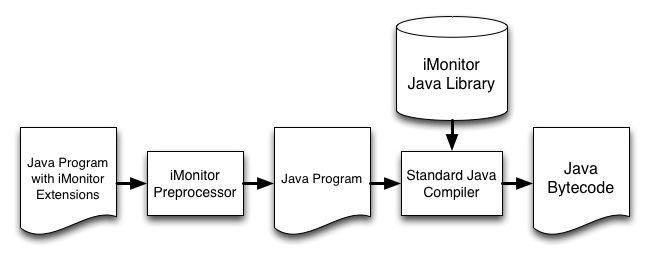
\includegraphics[width=70mm]{fig/flow.png}
  \caption{The framework of iMonitor}
  \label{fig:framework}
\end{figure}



\section{Details of iMonitor Implementation}
The implementation of the implicit-signal monitor in iMonitor involves four 
parts:
\begin{enumerate}
  \item Monitor-constructor: the constructor of the monitor class, including 
    definitions and declarations of additional variables to provide mutual 
    exclusion and synchronization of monitor. 
  \item Monitor-function entry: executed before each member function, 
    involving declarations of additional variables and code to maintain
    mutual exclusion of monitor. 
  \item Monitor-waituntil statement: including declarations of additional
    variables and signal/await statements to implement the waituntil.
  \item Monitor-function leave: executed before the return statement of 
    each member function, involving code to guarantee mutal exclusion and 
    synchronization of monitor. 
\end{enumerate}
The implementation of iMonitor is summarized in Table \ref{tab:iMonitor_imp}



\subsection{Naive}

\begin{SaveVerbatim}{NaiveConstructorImp}
Lock mutex;
Condition cond;
\end{SaveVerbatim}

\begin{SaveVerbatim}{NaiveEntryImp}
mutex.lock();
\end{SaveVerbatim}

\begin{SaveVerbatim}{NaiveWaituntilImp}
if(!C) {
  cond.signalAll();
  do {
    cond.await();
  } while(!C);
}
\end{SaveVerbatim}

\begin{SaveVerbatim}{NaiveExitImp}
mutex.unlock();
cond.signalAll();
\end{SaveVerbatim}

\begin{SaveVerbatim}{NConditionConstructorImp}
Lock mutex;
HashSet<AssertionConditionPair> setPairs;
create AssertionConditionPair for each global predicate and put them into setPairs;
\end{SaveVerbatim}

\begin{SaveVerbatim}{NConditionWaituntilImp}
if(C is local predicate) {
  create AssertionConditionPair for C and put them into setPairs;
} 
if(!C) {
  for(AssertionConditionPair pair : setPairs) {
    pair.conditionalSignal();
  }
  do {
    await();
  } while(!C); 
}

\end{SaveVerbatim}

\begin{SaveVerbatim}{NConditionExitImp}
if(setPairs != null) {
  for(AssertionConditionPair pair : setPairs) {
    pair.conditionalSignal();
  }
}
remove all local predicate in setPairs;
mutex.unlock();
\end{SaveVerbatim}

\begin{table*}
  \center
  \begin{tabular}{| l || l | l | }
    \hline
                & Naive & N-Condition\\
    \hline
    \hline
    Constructor & \BUseVerbatim{NaiveConstructorImp} 
                & \BUseVerbatim{NConditionConstructorImp} \\
    \hline
    Entry       & \BUseVerbatim{NaiveEntryImp} 
                & \BUseVerbatim{NaiveEntryImp} \\
    \hline
    Waituntil C & \BUseVerbatim{NaiveWaituntilImp} 
                & \BUseVerbatim{NConditionWaituntilImp} \\
    \hline
    Exit        & \BUseVerbatim{NaiveExitImp} 
                & \BUseVerbatim{NConditionExitImp} \\
    \hline
  \end{tabular}
  \caption{iMonitor implementation}
  \label{tab:iMonitor_imp}
\end{table*}

In the implementation of naive implicit-signal monitor, one lock variable, 
$mutex$, is declared for mutual exclusion, which should be acquired in 
the begining of every member function and released before the return statement.
In addition, one condition variable, $cond$, is declared for 
synchronization, on which the implementation of waituntil depends. In the 
waituntil statement the predicate expression is checked initially. If the 
expression is false; then all other threads which are waiting on $cond$ are 
signaled to reevaluate their predicate expression since the monitor state may 
change. The currenet thread then is blocked in a loop and reevaluate its 
predicate expression when it is signaled. On the exit of a member function, 
all threads waiting on $cond$ are signaled to reevaluate their preidcate 
expression since the monitor state may change. 

\subsection{N-Condition}

\subsection{HashMap-Condition}
\subsection{Dependent-Condition} 
\section{Experimental Results}
\subsection{Bounded-Buffer Problem}
\subsection{Reader/Writer Problem}
\subsection{Dining Philosophers  Problem}
\subsection{Sleeping Barber Problem}
\subsection{Access Patterns}

\section{Conclusions}

\appendix
\section{Appendix Title}

This is the text of the appendix, if you need one.

\acks

Acknowledgments, if needed.

% We recommend abbrvnat bibliography style.

\bibliographystyle{abbrvnat}

% The bibliography should be embedded for final submission.

\begin{thebibliography}{}
    \softraggedright

  \bibitem[Buhr et~al.(2005)Buhr, P.A.]{bh05}
    Buhr, P. A. and Harji, A. S. Implicit-Signal Monitors. ACM Transactions on Programming Languages and Systems, 27(6), 1270�1343. ACM. doi:10.1145/1108970.1108975

\end{thebibliography}

\end{document}
